\section*{Introduction}

The article that is the subject of this reproduction attempt was my first publication for which I provided code as supplementary material \cite{HinsenStructuralflexibilityproteins2008}. In computational biophysics, that was uncommon back in 2008, and unfortunately it remains the exception until today. The code consisted of two Python scripts plus instructions and was meant to help readers with applying the methods discussed in the article to different proteins, rather than ensure reproducibility which at that time I had never heard of. This explains why the supplied code does not reproduce the figures shown in the paper, but merely produces data files in plain text format, from which the plots were originally assembled by hand and by additional scripts that I did not consider worthy of publication.

\section*{Historical context}

The work described in the original article was performed in summer 2007. The scripts make heavy use of two libraries of which I am the principal author: the Molecular Modeling Toolkit (MMTK) \cite{Hinsenmolecularmodelingtoolkit2000}, then at version 2.5, and ScientificPython, then at version 2.7. These two libraries, first published in 1997, are among the oldest scientific computing packages in the SciPy ecosystem. They were initially written on the basis of Numerical Python \cite{DuboisNumericalPython1996}, the original array package for Python that was published in 1995. With the transition of the ecosystem to its successor NumPy \cite{OliphantguideNumPy2006}, initially released in 2006, I ported MMTK and ScientificPython using NumPy's compatibility module called \texttt{oldnumeric}. This combination was used for the original work, but unfortunately I did not write down the exact version of NumPy. My instructions recommend ``Numerical Python 23.8.2 or NumPy 1.x'', which turned out to be overly optimistic: NumPy is still in the 1.x version range, but frequent breaking changes make it impossible to run my code with recent NumPy releases. In fact, with version~1.9 NumPy removed the \texttt{oldnumeric} interface, breaking all of my molecular simulation code. I had envisaged to port the code to the official NumPy API, but decided not to do so because of the high risk of introducing errors. There are in fact several subtle changes in the API, such as using the transpose of a matrix compared to the original Numeric API, which are easy to overlook because incorrect use yields an incorrect result but no error message. With the end of support for Python~2, there is no longer any point in such a change, as it makes little difference if my code depends on one or two unmaintained software packages.

The remaining dependencies turned out to be less critical. netCDF, which my scripts use for data storage, was at version 3.4, but any more recent version can be substituted. Python itself, then at version 2.5, caused no problems either up to release 2.7. Python~3 is from my point of view a different language, the two major changes for scientific computing being a very different C API layer and a different definition of division. Porting would involve a significant amount of work because of the large number of extension modules in MMTK, most of which are C code hand-written for the C~API of Python 1.4, long before Pyrex \cite{EwingPyrex2010} and then its fork Cython \cite{BehnelCythonBestBoth2011} introduced more convenient ways to write extension modules.

\section*{Reproduction}

The \href{https://github.com/khinsen/rescience-ten-year-challenge-paper-3}{GitHub repository for this reproduction} contains all the code, input data, and instructions for running the reproduction on a modern GNU/Linux system with the Guix package manager \cite{CourtesReproducibleUserControlledSoftware2015,WurmusPiGxreproduciblegenomics2018}. It also lists the exact version numbers of all the software involved in the reproduction. For the numerical calculations alone, i.e. excluding the less critical tasks of downloading files and generating plots, a total of 254 Guix package must be rebuilt identically to guarantee bit-for-bit reproduction of the results.

\subsection*{Finding the code and the input data}

The project-specific scripts are still available for download from the journal's Web site. A copy can be found in the directory \scalebox{.7}[1.0]{\texttt{scripts-from-suplementary-material-to-original-paper}} of the code repository for this article. The directory \scalebox{.7}[1.0]{\texttt{updated-scripts-from-obsolete-web-server}} contains updated versions of the scripts, added for completeness. They were available from my laboratory's Web site for a few years, and contain minor improvements that are not relevant for this reproduction attempt, see the file \texttt{notes.org} for details. In the following, I use the original scripts.

All the dependencies have been available in public version-controlled repositories for many years. Obtaining the published code is therefore not a problem. The additional scripts that generated the original plots were not published as explained in the introduction. They have not survived two changes of computers. I still have backups that should contain them, but I have not been able to find a working reader for the DAT/DDS tapes on which these backups are stored. Another backup on a CD-ROM turned out to be unreadable.

The input data for reproducing the figures in the original paper consists of three protein structures from the Protein Data Bank (PDB) \cite{wwPDBconsortiumProteinDataBank2019}. The PDB updates its files from time to time. The file for a specifc entry is intended to represent the original data deposited by its authors, but may be modified to conform to newer versions of the file format, or to fix technical mistakes. There is thus no guarantee that a file downloaded today is the same as in 2008, but the scientific information it contains is supposed to stay the same. In practice, PDB updates have occasionally broken analyses of the annotations they contain, but not analyses of the original experimental data.

\subsection*{Running the scripts using the Guix package manager}

My preferred software management tool for reproducible computations is the Guix package manager \cite{CourtesReproducibleUserControlledSoftware2015}, which permits the bit-for-bit reconstruction of software environments at any later time. All the required dependencies have already been packaged in Guix, but since Guix only started in 2012, and the Python ecosystem was added even later, the original software versions of 2008 are not available.

The two scripts are meant to be run in sequence, once for each protein structure and crystal size. The first script, \texttt{calculate\_crystal\_fluctuations.py}, computes the normal modes of the crystal and stores them in a netCDF file. The second script, \texttt{analyze\_crystal\_fluctuations.py} extracts the relevant data for the plots from the netCDF file and writes them to text files.

Using the dependencies as defined in Guix in January~2020 (more precisely: commit \texttt{7357b3d7a52eb5db1674012c50d308d792741c48}), the first script runs without any apparent problem, but the second one crashes with an error message. This is the consequence of a breaking change in NumPy which modified the rules for the conversion of sequence-like Python objects into arrays. This problem can be fixed by changing a single line of code; however, neither the diagnosis nor the correction are likely to be obvious to someone who is not intimately familiar with NumPy.

I explored the possibility of using an earlier NumPy release in order to run the scripts unmodified. From the release history that is available on NumPy's GitHub repository, it appears that release 1.0.4 was current at the time of submission of my paper in late 2007. Unfortunately, this NumPy release cannot be installed with Python 2.7 because NumPy is distributed with a modified version of the \texttt{distutils} package. \texttt{distutils}  reads a configuration file produced during the installation of Python, whose format has changed between Python 2.5 and 2.7. I briefly envisaged installing Python 2.5, but that would have required backporting the modifications made for Guix, which seemed an unreasonable effort for performing a simple test.

In addition to the fix described above, I modified my scripts for convenience, making them read their originally hard-coded input parameters from  command line arguments instead. In fact, the scripts I had used for the original work also accepted command line arguments, but I had hard-coded them in the published versions in order to simplify the usage instructions.

\subsection*{Reproducing the figures}

As explained in the introduction, my goal with publishing the code of my computations was to enable reuse, not reproducibility. The code therefore does not reproduce the full figures, which need to be re-generated by hand from the numerical output. I have limited myself to producing figures that are similar enough to the originals to convince the reader that the results have been reproduced correctly. I also used different plotting software, Gnuplot \cite{WilliamsGnuplot2020}, in replacement of the originally used Grace \cite{GraceDevelopmentTeamGrace2008} which has not yet been packaged for Guix.

Figure~1 of the original publication does not contain any computed data and has therefore not been reproduced. The data it shows comes directly from the Protein Data Bank.

\begin{figure}
\caption{Blank figure included for aligning the figure numbers in this reproduction with the figure numbers in the original paper.}
\label{fig1}
\end{figure}

Figures~2 and~3 of the original publication compare ``single molecule'' to ``crystal'' results for two proteins. Only the latter are computed by the scripts in the supplementary material, and are shown in Figs.~\ref{fig2} and~\ref{fig3}. The ``single molecule'' curves were obtained by a script that was not published, and which I have lost. It would not be difficult to replicate, but that is not the goal of this reproduction attempt.

\begin{figure}
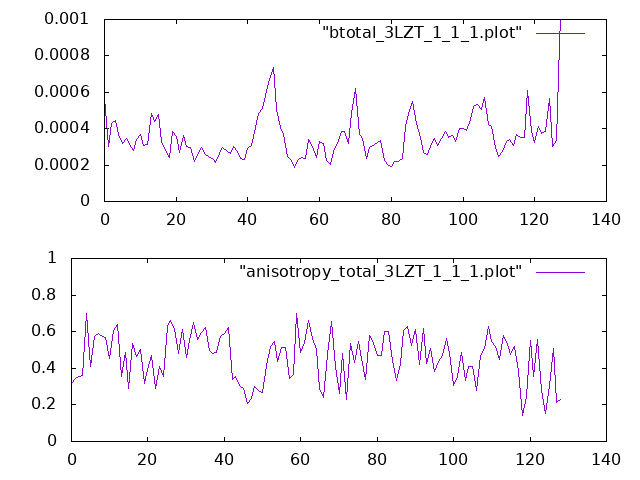
\includegraphics[width=.9\textwidth]{../reproduction/fig2.png}
\caption{Reproduction of Fig.~2 in the original publication.}
\label{fig2}
\end{figure}

\begin{figure}
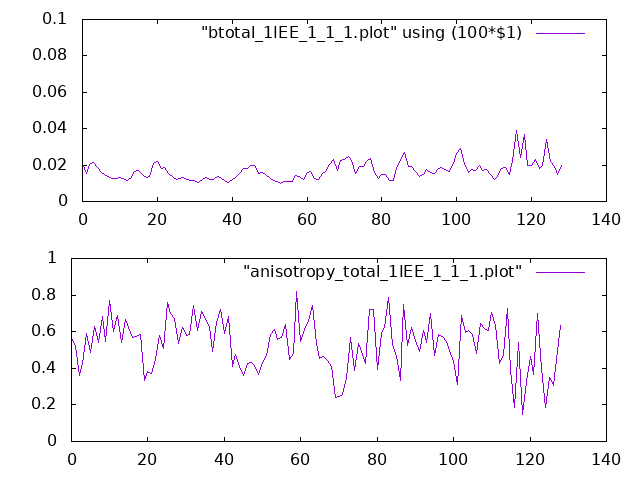
\includegraphics[width=.9\textwidth]{../reproduction/fig3.png}
\caption{Reproduction of Fig.~3 in the original publication.}
\label{fig3}
\end{figure}

Figure~4 of the original publication shows the dispersion relations for four different directions of wave propagation in the crystal. Unfortunately, the supplied scripts only produce a single file with points on the dispersion plots from all directions combined. The additional script required to separate these points by direction was not published and has been lost. The dashed lines labelled ``elastic medium'' were also computed by unpublished and lost scripts. Fig.~\ref{fig4} shows unconnected points that each lie on one of the drawn-out lines of the original Figure~4.
\begin{figure}
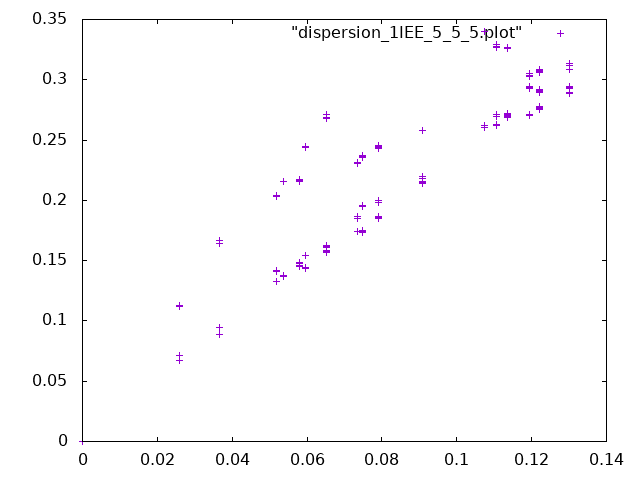
\includegraphics[width=.9\textwidth]{../reproduction/fig4.png}
\caption{Reproduction of Fig.~4 in the original publication.}
\label{fig4}
\end{figure}

Figure~5 of the original publication is reproduced almost entirely in Fig.~\ref{fig5}. One curve from the original plots, labelled ``extrapolation'', is missing because the script used for doing the extrapolation was not published and has been lost.
\begin{figure}
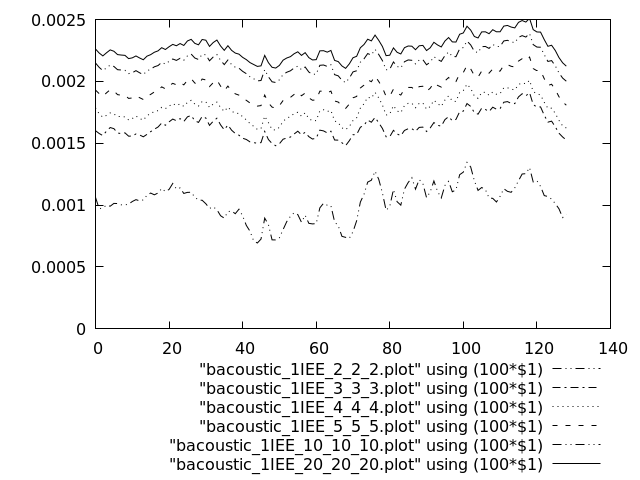
\includegraphics[width=.9\textwidth]{../reproduction/fig5a.png}
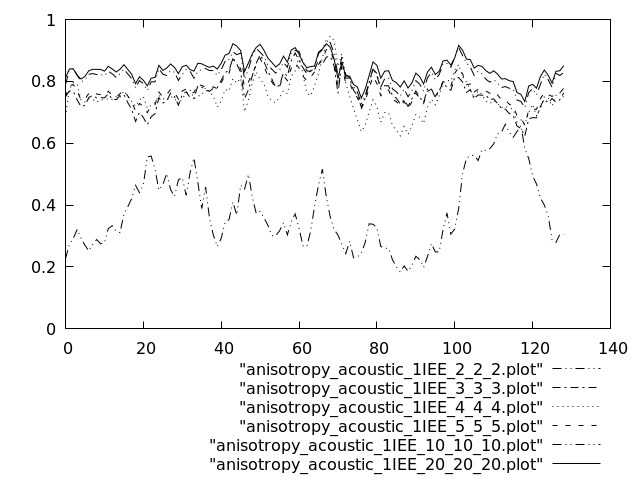
\includegraphics[width=.9\textwidth]{../reproduction/fig5b.png}
\caption{Reproduction of Fig.~5 in the original publication.}
\label{fig5}
\end{figure}

Finally, Figure~6 of the original publication has not been reproduced. It contains one curve each from Figs.~\ref{fig2} and~\ref{fig3}, combined with experimental data from the Protein Data Bank and a scaled curve using a scaling factor computed by yet another script that was not published and has been lost.

\section*{Conclusion}

The goal of this reproduction attempt was to answer three questions:
\begin{enumerate}
\item Can the code published in 2008 still be run today?
\item Does it produce results equivalent to those shown in the original figures?
\item Does the code fully reproduce the original results?
\end{enumerate}

My answers are
\begin{enumerate}
\item Yes, but only using obsolete versions of dependencies and after modification due to a breaking change in one of them.
\item Yes.
\item No, because not all the required code was published, and the unpublished code has been lost in the meantime.
\end{enumerate}

The obvious lesson for the future to draw from this exercise is the importance of publishing all the code, up to the automatic generation of figures and tables. Another regrettable omission I made in 2008 is not writing down the precise version numbers of all the code involved. It might have been useful in this case to know the precise version of NumPy used in the original work. In fact, my claim that the modification to a script was required as a consequence of a breaking change in NumPy is based merely on my memories and notes from other projects in which I had to make similar changes.

The final lesson would have to be drawn by a wider community of scientific software developers: breaking changes in widely used infrastructure code such as NumPy can cause a lot of damage in terms of lost reproducibility that may be difficult to diagnose and fix for someone else than the original authors. The open question that the scientific community has to figure out is where to place reproducibility on our scale of values, and for which time spans we consider it desirable. Structural biology is a methodologically mature domain of research, in which the main source of progress is not disruptive new methods, but incremental improvements of existing methods in the course of ongoing applications to biologically relevant systems. This is in fact the norm in science and technology \cite{Arthurnaturetechnologywhat2009}. In this context, my methodological work published in~2008 is by no means outdated. The last time I have referred to it myself (in so-far unpublished work) was in 2018. Reproducibility lifetimes of just a few years, corresponding to the current habits in the scientific Python ecosystem, are therefore problematic.

% NumPy's predecessor \texttt{Numeric} \cite{DuboisNumericalPython1996} used a semantic versioning scheme, and progressed from its first stable version~1 (released in March 1998) to version~24 in its decade of active development. Nevertheless, the changes in the major version number mostly reflected important new features. Backwards incompatible changes were, according to my memories, rare \footnote{Unfortunately the source code, and thus the release notes, for Numerical Python versions before~16 (first one to be published on SourceForge) is probably lost forever.} Today's NumPy started out as a merger of Numeric with an incompatible fork called \texttt{numarray}. 

\vspace{3mm}

The two pieces of software whose evolution has most impacted this work, Python and NumPy, deserve a more detailed discussion because of their importance in today's scientific computing. In the 12~years since the publication of my original paper, both have changed in a way that breaks compatibility with earlier version, causing software collapse \cite{HinsenDealingSoftwareCollapse2019} that has affected not just my two scripts, but much scientific software. However, the stories of the two pieces of software are also very different.

\vspace{1mm}

The Python language, first published in~1991, has evolved with no major compatibility issues up to its version~2.7, released in~2009 and maintained for another ten years \cite{WikipediacommunityHistoryPython2020}. This was largely the result of an unwritten policy decided by Python's ``benevolent dictator for life'', Guido van Rossum, who had the last word on all strategic decisions. However, new requirements due to changes in computing technology, in particular full Unicode support, turned out to be impossible to implement without breaking changes to the language. Van Rossum decided to make a one-time major revision of his language, both to address such fundamental issues and a large number of minor ones that had accumulated over time. The new language, Python~3, was first published in~2008 and was supposed to co-exist with Python~2 for a transition time of one decade. In retrospect, van~Rossum and his core developer team seriously underestimated the impact of this decision, which was unprecedented and turned out to become the most destructive event in the history of Open Source software.

The Python development team has officially ended support for Python~2.7 at the end of~2019, and its future is unclear at this time. Without maintenance, Python~2.7 is likely to remain usable for a few more years, before changes in operating systems, compilers, and Python's own dependencies will require adaptation. As noted by Rougier \cite{RougierRpLoupe2019}, ``this end of life might be a good thing for science because we now have at our disposal an advanced programming language that is guaranteed not to evolve anymore (i.e. Python 2.7)''. An important open question is whether someone else will take over maintenance of Python~2, which is always a possibility with Open Source software. The importance of Python~2 in the commercial sector (e.g. banks) makes this an economically viable possibility. Another important open question is how software distributions (Linux distributions but also platform-neutral distributions such as Anaconda \cite{AnacondaInc.Anacondasoftwaredistribution2020}) will react. They have an interest in removing Python~2 in order to reduce their own workload, and they may also do so for fear of security issues that won't be fixed any more. On the other hand, if user demand for software dependent on Python~2 is large enough, they may work out a compromise (such as offering Python~2 without networking modules), or take up minimal maintenance of Python~2 themselves.

\vspace{1mm}

NumPy was first published in 2006 as the merger of its direct predecessor, \texttt{Numeric} \cite{DuboisNumericalPython1996}, and an alternative array implementation called \texttt{numarray} that was optimized for large datasets \cite{GreenfieldnumarrayNewScientific2003}. Unlike Python, it has never had a clearly defined policy on backwards compatibility, and many breaking changes have happened in between the initial version~1.0 and today's version~1.18. It also differs from Python in having a much narrower application domain and thus a much smaller developer community. In 2018, an explicit policy about backwards compatibility was proposed as NumPy Enhancement Proposal \#23 \cite{GommersNEP23Backwards2018},
% https://numpy.org/neps/nep-0023-backwards-compatibility.html
% https://github.com/numpy/numpy/blob/a9bb517554004cf2ce7a4be93bcbfb63ee149844/doc/neps/nep-0023-backwards-compatibility.rst
which has so far been neither accepted nor rejected. If accepted, it would increase code stability because it is stricter in many ways than the \textit{ad hoc} decisions made in the past. However, the proposed policy states that ``Backwards incompatible changes can be made, provided the benefits outweigh the costs'', where the major cost is breaking user code. The proposal adds that ``Benefits include improved functionality, usability and performance (in order of importance), as well as lower maintenance cost and improved future extensibility.'' The decision whether benefits outweigh the costs, like all major decisions concerning NumPy, is made by ``consensus of all interested contributors'' \cite{NumPydevelopersNumPyprojectgovernance2020}.
 % https://docs.scipy.org/doc/numpy/dev/governance/governance.html
% https://github.com/numpy/numpy/blob/a9bb517554004cf2ce7a4be93bcbfb63ee149844/doc/source/dev/governance/governance.rst
While contributors are in a good position to judge the benefits, there is little reason to believe that they can fully appreciate the costs, which are borne by the users. Given the small size of the development team and the large user base, there is not much reason either to believe that the former group is representative for the latter one.

This reproducibility challenge highlights another issue that Open Source communities seem to be largely unaware of. What they consider their users are people interacting directly with their software. For NumPy, that's people who write Python code starting with \texttt{import numpy}. Developers silently expect such users to maintain their software, and in particular adapt it to breaking changes in dependencies. Whether or not this is a reasonable expectation is debatable. Making it silently certainly isn't. But more importantly, for infrastructure software such as NumPy, there is a vastly larger group of second or higher degree users, which includes scientists who want to build on the code that I published in 2008 with my original paper. Such users are unlikely to have the technical competence and the willingness to do software archaeology, i.e. read the release notes of all the dependencies of the software they use. A first step to help such users would be clearer communication about breaking changes. In 2017, I made a request to the NumPy community to adopt semantic versioning in order to permit packagers, application developers, and end users to identify backwards-incompatible changes more easily. After a heated discussion \cite{NumPydevelopersandusersRequestusesemantic}, the request was rejected, the main arguments being that (1) semantic versioning is not common in the Python ecosystem, (2) it would cause version numbers to increase too rapidly.

\vspace{3mm}

Ultimately, the increasingly common phenomenon of software collapse in scientific computing is due to a lack of coordination between the needs of developers and users, which in turn is a consequence of the failure of the scientific community to take care of its software infrastructure. Young scientists and engineers join Open Source communities, mostly as unpaid volunteers, to improve software for the use cases they have encountered in their own work. Maintaining infrastructure over longer time spans for a wide user base requires dedicated personnel under the supervision of experienced research software engineers. It requires institutions that have infrastructure maintenance as their main objective. As long as such institutions do not exist, computational scientists will have to work around software collapse if the software they use evolves on a faster time scale than their scientific methods, as I have shown in this reproduction work using Guix.
